% This is "sig-alternate.tex" V2.0 May 2012
% This file should be compiled with V2.5 of "sig-alternate.cls" May 2012
%
% This example file demonstrates the use of the 'sig-alternate.cls'
% V2.5 LaTeX2e document class file. It is for those submitting
% articles to ACM Conference Proceedings WHO DO NOT WISH TO
% STRICTLY ADHERE TO THE SIGS (PUBS-BOARD-ENDORSED) STYLE.
% The 'sig-alternate.cls' file will produce a similar-looking,
% albeit, 'tighter' paper resulting in, invariably, fewer pages.
%
% ----------------------------------------------------------------------------------------------------------------
% This .tex file (and associated .cls V2.5) produces:
%       1) The Permission Statement
%       2) The Conference (location) Info information
%       3) The Copyright Line with ACM data
%       4) NO page numbers
%
% as against the acm_proc_article-sp.cls file which
% DOES NOT produce 1) thru' 3) above.
%
% Using 'sig-alternate.cls' you have control, however, from within
% the source .tex file, over both the CopyrightYear
% (defaulted to 200X) and the ACM Copyright Data
% (defaulted to X-XXXXX-XX-X/XX/XX).
% e.g.
% \CopyrightYear{2007} will cause 2007 to appear in the copyright line.
% \crdata{0-12345-67-8/90/12} will cause 0-12345-67-8/90/12 to appear in the copyright line.
%
% ---------------------------------------------------------------------------------------------------------------
% This .tex source is an example which *does* use
% the .bib file (from which the .bbl file % is produced).
% REMEMBER HOWEVER: After having produced the .bbl file,
% and prior to final submission, you *NEED* to 'insert'
% your .bbl file into your source .tex file so as to provide
% ONE 'self-contained' source file.
%
% ================= IF YOU HAVE QUESTIONS =======================
% Questions regarding the SIGS styles, SIGS policies and
% procedures, Conferences etc. should be sent to
% Adrienne Griscti (griscti@acm.org)
%
% Technical questions _only_ to
% Gerald Murray (murray@hq.acm.org)
% ===============================================================
%
% For tracking purposes - this is V2.0 - May 2012

\documentclass{sig-alternate}

\pdfpagewidth=8.5in
\pdfpageheight=11in

\usepackage{lmodern}
\usepackage{amsmath}
\usepackage{booktabs, multicol, multirow}
\usepackage{verbatim}
\usepackage{enumerate}
\usepackage{hyperref}
\usepackage{subfigure}
\usepackage{color}
\usepackage[linesnumbered,ruled,vlined]{algorithm2e}
\usepackage{url}
\usepackage{listings}
\usepackage[T1]{fontenc}
\usepackage{xcolor}
\lstset{escapeinside={<@}{@>}}
\usepackage{rotating}
\usepackage{cite}
%\usepackage{caption}


\definecolor{dkgreen}{rgb}{0,0.6,0}
\definecolor{gray}{rgb}{0.5,0.5,0.5}
\definecolor{mauve}{rgb}{0.58,0,0.82}
\definecolor{light-gray}{gray}{0.8}

\lstset{
  frame=none,
  language=C,
  aboveskip=3mm,
  belowskip=3mm,
  showstringspaces=false,
  columns=flexible,
  basicstyle={\small\ttfamily},
  %numbers=left,
  %numberstyle=\tiny\color{gray},
  keywordstyle=\color{blue},
  commentstyle=\color{dkgreen},
  stringstyle=\color{mauve},
  breaklines=true,
  breakatwhitespace=true
  tabsize=3
}

\begin{document}
%
% --- Author Metadata here ---
%\conferenceinfo{ASE}{'97 El Paso, Texas USA}
%\CopyrightYear{2007} % Allows default copyright year (20XX) to be over-ridden - IF NEED BE.
%\crdata{0-12345-67-8/90/01}  % Allows default copyright data (0-89791-88-6/97/05) to be over-ridden - IF NEED BE.
% --- End of Author Metadata ---

\title{ConAir: A Lightweight Concurrenty Bug Recovery Tool}
%\subtitle{[Extended Abstract]
%\titlenote{A full version of this paper is available as
%\textit{Author's Guide to Preparing ACM SIG Proceedings Using
%\LaTeX$2_\epsilon$\ and BibTeX} at
%\texttt{www.acm.org/eaddress.htm}}}
%
% You need the command \numberofauthors to handle the 'placement
% and alignment' of the authors beneath the title.
%
% For aesthetic reasons, we recommend 'three authors at a time'
% i.e. three 'name/affiliation blocks' be placed beneath the title.
%
% NOTE: You are NOT restricted in how many 'rows' of
% "name/affiliations" may appear. We just ask that you restrict
% the number of 'columns' to three.
%
% Because of the available 'opening page real-estate'
% we ask you to refrain from putting more than six authors
% (two rows with three columns) beneath the article title.
% More than six makes the first-page appear very cluttered indeed.
%
% Use the \alignauthor commands to handle the names
% and affiliations for an 'aesthetic maximum' of six authors.
% Add names, affiliations, addresses for
% the seventh etc. author(s) as the argument for the
% \additionalauthors command.
% These 'additional authors' will be output/set for you
% without further effort on your part as the last section in
% the body of your article BEFORE References or any Appendices.

\numberofauthors{2} %  in this sample file, there are a *total*
% of EIGHT authors. SIX appear on the 'first-page' (for formatting
% reasons) and the remaining two appear in the \additionalauthors section.
%
\author{
  % You can go ahead and credit any number of authors here,
  % e.g. one 'row of three' or two rows (consisting of one row of three
  % and a second row of one, two or three).
  %
  % The command \alignauthor (no curly braces needed) should
  % precede each author name, affiliation/snail-mail address and
  % e-mail address. Additionally, tag each line of
  % affiliation/address with \affaddr, and tag the
  % e-mail address with \email.
  %
  % 1st. author
  \alignauthor Shiyu Dong\\
  \affaddr{The University of Texas at Austin}\\
  \email{shiyud@utexas.edu}\\
  % 2nd. author
  \alignauthor Xuebin Yan\\
  \affaddr{The University of Texas at Austin}\\
  \email{annyan@utexas.edu}\\
}
% There's nothing stopping you putting the seventh, eighth, etc.
% author on the opening page (as the 'third row') but we ask,
% for aesthetic reasons that you place these 'additional authors'
% in the \additional authors block, viz.
% Just remember to make sure that the TOTAL number of authors
% is the number that will appear on the first page PLUS the
% number that will appear in the \additionalauthors section.

\maketitle
\begin{abstract}
Concurrency bugs are usually hidden in software and is not really easy to be
exposed. These bugs often causes severe failure to end-users but they are
usually hard to fix by developers. ConAir~\cite{zhang2013conair} is a tool
targeting on recover and fix concurrent bugs for end users. It is based on two
observations that rolling back a single thread by re-executing idempotent region
for that thread is enough for recovering many of the concurrent bugs.

In this project we build and run ConAir from source code provided by the author.
Experiments from the authors of ConAir shows that ConAir is capable to fix and
recover concurrency bugs in many real life programs with different sizes, and
our own experiment results demonstrate that other than recovering the known four
types of concurrency bugs, ConAir has potential to fix more unknown types of
bugs.
\end{abstract}


%A category including the fourth, optional field follows...
\category{D.1.3}{Programming Techniques}{Concurrent Programming}
% A category with the (minimum) three required fields
\category{D.2.5}{Software Engineering}{Testing and Debugging}
\category{D.4.1}{Operating Systems}{Process Management}


\keywords{idempotency, concurrency bugs, failure recovery, static analysis, bug
fixing}

\pagenumbering{arabic} \setcounter{page}{1}
\chapter{Introduction}


\section{Background}
Information explosion is a term that describes the rapidly
increasing amount of published information and the effects of this
abundance of data. As the amount of available data grows, the
effective and efficient management of the information becomes more
difficult, leading to information overload or information fatigue.
The explosion problem of video data, in particular, posts more
technical challenges due to the fact that audio-visual features are
unorganized and unordered in nature. Video retrieval, aiming to mine
and search semantic knowledge from an over-abundance of video
dataset, has drawn increasing attentions from both extant web search
engines (e.g., Yahoo!, Google and so on) and scientific researchers.
However, the video usually carries a versatile semantic message
which has immediate meaning for a human. But for a computer, it is
far from the truth. This discrepancy between the machine computable
low-level features and its semantic interpretation by human subjects
is commonly referred to as the \emph{semantic gap}
\cite{ArnoldW.M.Smeulders:IEEETPAMI:2000}. Bridging semantic gap has
long been recognized as a key factor in enabling semantic-based
video retrieval.

Early efforts aiming to bridge the semantic gap focused on the
feasibility of mapping low-level features, e.g. color, pitch and
texture, directly to high-level semantic concepts such as commercial
\cite{R.Lienhart:IEEECMCS:1997}, nature \cite{J.R.Smith:IEEEMM:1997}
and baseball \cite{Y.Rui:ACMM:2000}. Many dedicated detectors have
been developed for this intuitive purpose, which map low-level
features to single semantic concept based on simple decision rules.
The detector-specific-approaches, however, become impractical and
intractable with the demand of large-scale automatic annotation of
video archives. It is almost impossible to develop a dedicated
detector for each possible concept, as there are just too many
concepts. Instead of developing concept-specific detectors, a recent
trend has therefore been shifting to develop generic detectors.
Specifically, with a set of concept-specific training examples,
generic detectors are trained separately with single approach
without considering concept-specific knowledge
\cite{MilindR.Naphade:IEEEICOME:2000,A.Amir:TRECVID:2003,C.G.M.Snoek:NISTTRECVID:2005}.
This has enlightened the possibility of developing large-scale
concept detectors, ending up a multimedia ontology suitable for both
video annotation and search.

The core of generic-based approaches mainly relies on the paradigm
of supervised learning \cite{CeesG.M.Snoek:ACMMM:2006}. The major
limitation, nevertheless, is the need of large amount of labeled
examples for training. The labeling of multimedia data is generally
a labor intensive, subjective and erroneous process. The researchers
have indeed looked forward a large shared annotation dataset for
concept detector learning. To cope with the demand, initiated by Lin
et al. \cite{C.Y.Lin:TRECVID:2003}, a common annotation effort was
recently started for the TREC Video Retrieval Evaluation (TRECVID
Workshop) 2005 benchmark. It has yielded a large accurate set of
groundtruth including a lexicon of 39 concepts
\cite{M.R.Naphade:2005}. Driven by this effort, various sets of
annotated concepts, such as Medmill's 101 machine-learned detectors
\cite{CeesG.M.Snoek:ACMMM:2006} and the recent collaborative
undertaking development of Large-Scale Concept Ontology for
Multimedia (LSCOM) \cite{Milind.Naphade:IEEEMM:2006}, have become
publicly available.

However, such a widely collaborative annotation effort, with such a
large amount of shared groundtruth, can never reach the richness of
human-know vocabularies. New concepts and new examples will have to
be annotated, when we face any new domain. More seriously, different
people tend to use different terms in annotating the same concept
during labeling, resulting in label ambiguity. Even for the same
user, he/she will trend to use different terms in different context.
To deal with this problem, ontologies
\cite{C.Fellbaum:1998,H.Liu:BTTJ:2004} were developed to structure
terms employed by user, which can make descriptions more consistent.
Exploiting ontology on video domain can embed the inherently
uncertain tagging, generated either by machine or human, in a
semantically rich context. With the multimedia ontology, we can
disambiguate various interpretations and find concepts that are more
general and useful for retrieval. As the video domain is broad and
in practice contains any topic, a large and domain independent
ontology is necessary.

\section{Ontology and Multimedia Ontology}
In philosophy, ontology is the study of the kinds of things that
exist. Ontologies are often said, colorfully,``to carve the world at
its joints". In information science, however, it is unrealistic,
when we realize that the world is too big to be carved. What we say
ontology is therefore referred to domain ontology, which describe
the body knowledge of a domain. Different from traditional domain
knowledge, an ontology analysis clarifies the structure of knowledge
by identifying the basic conceptualizations needed to talk about all
instances, recognizing their types, and relating the topology to
additional constraints. A well-structured knowledge representation
is easy to be shared with others who have similar needs in that
domain, thereby eliminating the need for replicating the
knowledge-analysis process. Shared ontologies can thus form the
basis for domain-specific knowledge-representation languages. In
contrast to the previous generation of knowledge-representation
languages (e.g KL-One \cite{R.J.Brachman:CS:1985}), these languages
are content rich; they have a large number of terms that embody a
complex content theory of the domain
\cite{B.Chandrasekaran:IEEEIS:1999}.

The current interest in ontologies come from the alternation of
focus between content theories and mechanism theories. Many
mechanisms, such as rule systems, frame languages, neural nets,
fuzzy logic, constraint propagation, or unification, are proposed as
exciting secret of making intelligent machines. With such wonderful
mechanisms, however, we cannot do much without a good content
theory. Moreover, we often recognize that once a good content theory
is reached, many different mechanisms might be used equally well to
implement effective systems, all using essentially the same content
\cite{B.Chandrasekaran:IEEEE:1994}. Ontologies are quintessentially
content theories. Thus far, they have played important roles in
information systems, natural language understanding (NLU) and
knowledge-based systems. In the domain of multimedia, ontology is
regarded as an emerging, yet natural, tool to bridge the semantic
gaps as a result of annotation ambiguity due to fuzziness of
audio-visual information. Ideally, ontology should be able to deal
with the richness of natural vocabularies, not only in textual but
also audio-visual domain.

Given the term Multimedia Ontology, people might usually refer to
some standard controlled vocabularies and classification schemes for
multimedia. For example, MPEG-7 has standardized more than 140
classification schemes that describe properties of multimedia
content. Similarly, TGM-I provides a large thesaurus for cataloging
graphical material. There are several multimedia controlled
vocabularies available. However, these standard schemes have
received little attention from the multimedia research community,
mostly because many of the terms in these schemes are not suitable
for automated tagging. For example, the MPEG-7 Genre Classification
Scheme (urn:mpeg:mpeg7:cs:GenreCS:2001), which is used to classify
programs based on their content or subject matter, defines terms
such as``special events" and``remarkable people." The terms might be
useful for classifying multimedia content but do not lend them well
to automated extraction. Such subjective concepts also make it
difficult for two annotators to completely agree, which further
complicates this issue. This highlights the third critical
requirement for the multimedia concept ontology: the feasibility of
automated extraction \cite{Milind.Naphade:IEEEMM:2006}.

Multimedia ontology helps to identify the body classes, their
properties and the relationship between them. It will provide the
reasoning strategy a well-structured knowledge base. On the other
side, the reasoning strategy also has impact on the development of a
multimedia ontology. We could in fact explain this in a common
sense: how we build a thing is strongly related with how we use it,
and vice versa.

\section{Concept-based Video Search and Ontology Reasoning}
Recent applications of using multimedia ontology are mainly for
concept-based video search, as illustrated in
Figure~\ref{fg-semantic_gap}.
%
The sensory gap from user queries to raw data is bridged with a pool
of concepts enriched with general-purpose vocabularies, for
instance, from ontology (e.g., WordNet) and external information
(e.g., Internet). Based on such concepts, a set of concept detectors
is developed to represent the high-level semantics. The detectors
are automatically learnt with training examples described by
multi-modality features. Given a user query, the best set of
concepts that can describe the semantic of query is reasoned through
the vocabularies. A search list is then produced by ranking items
(e.g., shots) according to their signal responses to the selected
concept detectors.
%
\begin{figure}[t]
\centering
\includegraphics[width=0.8\textwidth]{semantic_gap.eps}
\caption{General framework of concept-based video retrieval.}
\label{fg-semantic_gap}
\end{figure}
%

Under the concept-based retrieval framework as depicted in
Figure~\ref{fg-semantic_gap}, an apparent issue is that, given the
concept set, the mapping ambiguity between queries and concepts
needs to be carefully resolved. A common solution is to consider the
mapping through ontology reasoning
\cite{CeesG.M.Snoek:IEEETM:2006,Anthony.Hoogs:CVPR:2003,Alejandro.Jaimes:ICOIVR:2003,Yi.Wu:IEEEICOME:2004,M.R.Naphade:2005},
or more precisely selecting the concepts which minimize the
linguistic distance with query terms. The mapping is normally done
with the shared knowledge topology such as WordNet
\cite{C.Fellbaum:1998}. A fundamental question is: whether the
ontology reasoning can provide a common ground for the consistence
reasoning of concept similarities?
%
\begin{figure}
 \centering \subfigure[]
{\includegraphics[width=0.48\textwidth]{cfo.eps}\label{fig:cfo}}
 \centering \subfigure[]
{\includegraphics[width=0.48\textwidth]{OSS.eps}\label{fig:oss}}
%\subfigure[]
%{\includegraphics[width=0.24\textwidth]{os2mode.eps}\label{fig:os2}}
\caption{Reasoning with (a) ontology, reasoning is done in a
subgraph without a global view of the whole structure, (b) OSS,
concepts are projected into the space according to their relations
with selected vantage (basis) concepts.}\label{fig:CFO_OSS}
\end{figure}
%
Take Figure~\ref{fig:CFO_OSS}(a) as an example, let concepts $a$ to
$e$ as children and $v_1$ to $v_3$ as ancestors. Using ontology
reasoning approach such as Resnik \cite{Philip.Resnik:IJCAI:1995}
which measures similarity of two concepts with Information Content
(IC) \cite{Philip.Resnik:IJCAI:1995} of their nearest common
ancestor, the concept pairs $(a,b)$ and $(a,c)$ could have the same
similarity equals to IC of $v_1$, although $(a,c)$ sharing another
ancestor $v_2$ and intuitively should be more alike. In this case,
supposing $a$ is a query item, concept selection is hard to be made
between $b$ and $c$. On the other hand, the similarity scores of
$(d,e)$ and $(a,b)$ cannot be reasonably compared as they reside in
different parts of the ontology which carry different statistic and
structural information.
%
In brief, the reasoning is {\em locally} determined in a subgraph
without a global ontological view. Such mapping strategy indeed
causes the similarity scores of query terms and concepts not
directly comparable, resulting in less meaningful matching when
finding the ``best concepts'' to interpret query semantics.

\section{Ontology-enriched Semantic Space}
In this report, we propose a novel model called Ontology-enriched
Semantic Space (OSS) to enable the uniform and \emph{global}
comparison of concept pairs by providing a {\em computable}
platform. With reference to Figure~\ref{fig:CFO_OSS}(b), the
semantic space is represented as a linear space spanned with a set
of concepts enriched with ontology knowledge. These concepts of OSS
can be viewed as the ``vantage'' points
\cite{RobertoF.Santos.Filho:ICDE:2001,CaetanoTraina.Jr.:VLDB:2007}
\cite{Malcolm.Slaney:ICME:2002,A.Berenzweig:ICME:2003,Jules.Vleugels:PR:2002}
of the original ontology space. Supposing the ancestors $v_1$ to
$v_3$ of Figure~\ref{fig:CFO_OSS}(a) are selected as the vantage
concepts of OSS, then one can linearly project the concepts $a$-$e$
to the metric space according to their ontological relation with the
selected vantage concepts through conventional ontology reasoning.
Such framework indeed sights several opportunities. First, the
vantage concepts provide a high coverage of semantic space, and are
probably the ones that should be developed if they are feasible to
be built with the current technology. Secondly, in contrast to the
examples in Figure~\ref{fig:CFO_OSS}(a), the space guarantees
\emph{global} consistency in comparing the concept pairs like
$(a,b)$, $(a,c)$ and $(d,e)$.

An intuitive explanation of OSS is that the space is linearly
constructed to model the available set of concepts. The expressive
power of OSS is linguistically spanned with a set of vantage
concepts, which is easier to generalize, not only to the available
concept detectors but also to the unseen concepts.

%However, some of the vantage concepts of OSS may have inter-concept
%correlation, which causes their corresponding vectors are not
%strictly orthogonal to each other. This will bias the measurement of
%similarity. To solve this problem, we further model the
%orthogonality of semantic space, resulting in an Orthogonal
%Ontology-enriched Semantic Space ($OS^2$). In contrast to OSS,
%$OS^2$ performs spectral decomposition to transform the semantic
%space into a novel space with orthogonal base. With reference to
%Figure~\ref{fig:CFO_OSS}(c), the base ($B_1$, $B_2$ and $B_3$) in
%$OS^2$ are not formed by the real concepts. They are, however,
%linear combinations of basis concept vectors of OSS, and are more
%powerful in terms of expressive and generalization abilities for
%having the orthogonal property which optimally covers the semantic
%space. Thus a more consistent way of comparing concept similarity
%scores can be guaranteed in $OS^2$.

\section{Organization of This Report}
With OSS, we explore several search related tasks including concept
selection and detector fusion in this report. The major
contributions of our works are briefly summarized as follows:
%
\begin{itemize}
\item
{\em Scalability}: Building detectors for all concepts is impossible
and not necessarily \cite{A.Hauptmann:CIVR:2007,W.H.Lin:ICME:2006}.
A practical question is which detectors should be developed given
the information at hand. Compared to recent works in
\cite{W.H.Lin:ICME:2006}, OSS provides another novel view of
selecting concepts which have higher generalization ability in query
answering.


\item
{\em Query-concept mapping}: With OSS, the mapping is no longer a
local similarity comparison. Global consistency is ensured so that
the selection of concepts becomes meaningful.


\item
{\em Query disambiguation}: User queries are mostly ambiguous. We
explore OSS to predict the search intention by finding the exact
senses of query terms.
\end{itemize}

The remaining chapters are organized as follows.
Chapter~\ref{chp:related_work} briefly describes the current
state-of-the-art about multimedia ontology and concept-based video
search. Chapter~\ref{chp:modelingSS} presents the main idea of
modeling and constructing OSS. Chapter~\ref{chp:properties} analyzes
the properties of OSS. Finally, Chapter~\ref{chp:experiments}
presents experiments and Chapter~\ref{chp:conc} concludes this
report.

\section{ConAir Overview}
\label{chp:Overview}
\subsection {Two observations}
The design of ConAir is based on two ovservations:
\begin{itemize}
\item
Roll back a single thread is sufficient to recover from most concurrency-bug failures.
\item
Reexecute an idempotent region is sufficient to recover from many concurrency-bug failures.
\end{itemize}
\subsection{Observation I}
For most concurrency bugs, reexecuting one failing thread is sufficient to fix bugs.In the following part, most common concurrency bugs will be discussed separately:\\
\subsubsection{Recovering atomicity-violation bugs}
Atomicity violations contribute to about 70 \% of real-word non-deadlock bugs[].For read and write operations, there are four kinds of atomic violation operations, including Read after Write (RAW), Read after Read (RAR), Write after Read (RAW) and Write after Write (WAW). 
\begin{figure}
\begin{minipage}[t]{0.48\linewidth}
\centering
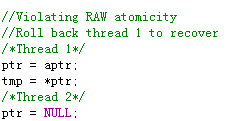
\includegraphics[width=\textwidth]{figs/RAW.png}
\caption{RAW atomic violation}
\label {RAW}
\end{minipage}%
\begin{minipage}[t]{0.48\linewidth}
\centering
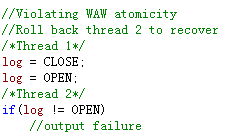
\includegraphics[width=\textwidth]{figs/WAW.png}
\caption{Violating WAW atomicity}
\label{WAW}
\end{minipage}
\end{figure}

\begin{figure}
\begin{minipage}[t]{0.48\linewidth}
\centering
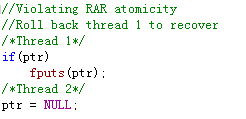
\includegraphics[width=\textwidth]{figs/RAR.png}
\caption{RAR atomic violation}
\label {RAR}
\end{minipage}%
\begin{minipage}[t]{0.48\linewidth}
\centering
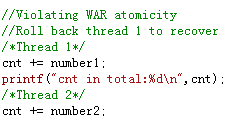
\includegraphics[width=\textwidth]{figs/WAR.png}
\caption{Violating WAR atomicity}
\label{WAR}
\end{minipage}
\end{figure}
As in Figure~\ref{RAW}, in thread 1, a global pointer is set to point to aptr and then, dereference it and give the value to a local variable tmp. In thread 2, the global pointer is initialized to NULL. Consider the situation that the first sentence of thread 1 is executed and then thread 2 is executed. When ptr is dereferenced and give its value to tmp, segamentation fault happens. In this case, roll back thread 1 until thread 2 finishes and do the given value part. The bug can be fixed.\\
As in Figure~\ref{WAW}, if thread 2 happens before the end of thread 1, error happens. In this case, rolling back thread 2 can fix the bug.\\
As in Figure~\ref{RAR} and Figure~\ref{WAR}, still rolling back one thread can fix the possible concurrency bugs. In general, for atomic violation bugs, rolling back one thread is sufficient to fix them.
\begin{figure}[t]
\centering
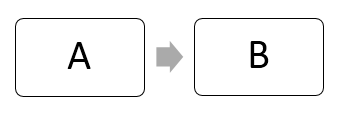
\includegraphics[width=0.5\textwidth]{figs/order_violation.png}
\caption{Order violation bug}
\label{order violation}
\end{figure}
\subsubsection{Recovering order-violation bugs}
Another kind of concurrency bug is called order-violation. That is one thread is required to be finished before another one. For example, in Figure~\ref{order violation}, A is required to finish before B. In this case, roll back B until A finishes can fix the bug.
\subsubsection{Rocovering deadlock bugs}
A very common concurrency bug in multi-thread programming is deadlock problem. As in Figure~\ref{deadlock}, thread A holds lock 1, thread B holds lock 2 and thread C holds lock 3. A still wants lock 2, while it's held by B. So A is blocked. Similar situation happens in B and C. In this case, roll back any thread can fix deadlock. If roll back B, B releases lock 2, so that C can finish and release lock 3 and 2. Then B can finish. Finally, A can get all resource it wants and finish itself.
\begin{figure}[t]
\centering
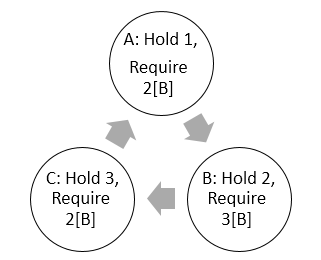
\includegraphics[width=0.5\textwidth]{figs/deadlock.png}
\caption{Deadlock}
\label{deadlock}
\end{figure}

\subsection{Observation II}
\label{sbii}
For observation II, it indicates that roll back certain area of one thread is sufficient to fix bugs and that area is defined as idempotent region.\\
\textbf{Idempotent region}:a code region that can be reexecuted for any number of times without changing the program semantics.\\
It should end before the failing point because it is meaningless to roll back the error part. Besides it, the idempotent region should not contain any writes to shared variables. If it is, roll back it will continously change a global variable, which is unwanted by users. Furthermore, it will not contain any I/O operations. According to investigation, only 15 \% concurrency bugs contain I/0 operation. In order to guarantee the performance of ConAir, I/O operation is eliminated from idempotent region. Also, it should not contain any writes to local variables that could cause incorrect execution. This rule is also added to guarantee the correnctness of the ConAir. Some local variables, such as static ones is initialized once and changed extends for the entire run of the whole program. If it is included in the idempotent region, potentially incorrect output may happen.\\
All rules are set to guarantee the correctness and performance of the usage of ConAir. Above all, the working principle of the ConAir is to roll back a single thread (failing thread) with its idempotent region.

 

\chapter{Design and Implementation of ConAir}
\label{chp:Design}
According to the working principle of ConAir, there are three main challenges of the design of ConAir. 
\begin{itemize}
\item
How to decide the failing point of the program
\item
How to find the idempotent region of the thread
\item
How to realize roll back step
\end{itemize}

\section{Infrastructure}
In this chapter we will discuss our infrastructure setup for building and
running ConAir, and the toolchain of using the ConAir tool.

\subsection{Infrastructure Setup}
One of the standards that was mentioned previously to evaluate the tool is
Compatibility, which means the tool should have no OS/hardware modification.
When we try to build and run the ConAir tool, however, we find out that although
it does not require any OS/hardware modification, it has very strong requirement
to the OS and corresponding software installed.

We make many effort in order to make ConAir compile and run. For example, We try
four different versions of Linux: Ubuntu 12.04 x64, Ubuntu 12.04 x86, the
Lonestar Cluster of UT, as well as CentOS 5.9. The first two are the OS that we
have as a virtual machine. None of them work perfectly. Then we ask the
author and they provide us the specific OS version that they use. Then we try
Lonestar Cluster which has an OS pretty similar to the one that the author
provides, but we do not have the privilege to install the required runtime
library. Finally we tried CentOS 5.9 which is exactly the same as the author
suggests, but we still cannot fix the compatibility issue (missing GLIBCXX\_3.4.9
and GLIBC\_2.7).

We also try different versions of LLVM, llvm-gcc and gcc. Specifically, we try
two versions of LLVM, llvm-2.8 and llvm 2.9; we try three versions of llvm-gcc:
the binary of llvm-gcc-4.2-2.8, binary of llvm-gcc-4.2-2.9, and llvm-gcc-4.2-2.8
built from source code; also we try five different versions of gcc: 4.7.3,
4.6.3, 4.4.3, 4.2.1 and 4.3.1 from source. For each try we do our best to remove
any compilation or dependency issue, and we try many combination between
different OS, LLVM, llvm-gcc and gcc. This process is very tedious and it take
more than 50\% of our time for this project. However, although we try very hard
we still cannot find a combination that is perfectly working. The main problem
we face is that the front end of LLVM cannot treat floating point global
variables appropriately. We believe that is because the version of LLVM we use
is too old, but ConAir does not support newer version of LLVM.

Fortunately, although we have the above issue, for normal multithread programs
without floating points we are able to make ConAir compile and run. Therefore we
can still do some experiments to demonstrate the effect of ConAir. We will show
our experiment results in section~\ref{sec:experiment}

\subsection{Toolchain}
There are several steps needed to make ConAir work, and
Figure~\ref{fig:toolchain} shows the structure of the ConAir ToolChain. Here we
want to generate two executables, the original one and the fixed one, so that we
can compare and see if the concurrency bugs have been fixed or not.\\
\begin{figure}[htbp]
\centering
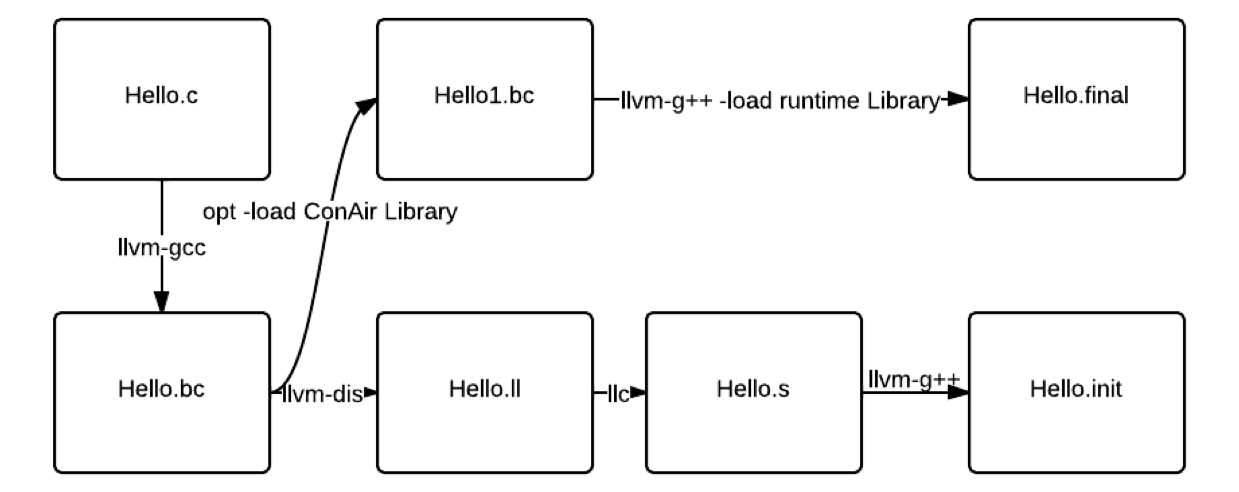
\includegraphics[width=0.5\textwidth]{figs/toolchain.png}
\caption{Toolchain of ConAir}
\label{fig:toolchain}
\end{figure}
\textbf{Generating the original executable}
In order to generate the original executable, we first use \textbf{llvm-gcc}, a
LLVM front end compiler, to compile the C source code \textit{Hello.c}, into
LLVM bitcode \textit{Hello.bc}. LLVM bitcode is a high level intermediate
representation (IR) of LLVM. It will unify source code in different languages
into a common source code, with no optimization applied.

After the LLVM bitcode is generated, we then use \textbf{llvm-dis}, a LLVM
disassembler, to disassemble the above bitcode into LLVM assembly code
\textit{Hello.ll}. After that, we will use \textbf{llc}, a static compiler of
llvm, to generate the above assembly code into another assembly code for a
specified architecture \textit{Hello.s}. Finally, we will use another front end
compiler \textbf{llvm-g++} to compile the above assembly code into the original
executable \textit{Hello.init}\\

\textbf{Generating the fixed executable}
In order to generate the fixed executable, we reuse the same bitcode
\textit{Hello.bc} above. We use LLVM \textbf{opt}, which is the LLVM optimizer,
to load the ConAir library first. This step will perform static code analysis of
the above bitcode, identify the failure site and idempotent region, and do the
code transformation by inserting setjump and longump to the failure site and
idempotent regions. All above process is done in the bitcode level, and in the
end it will generate a new bitcode called \textit{Hello1.bc}.

After the new bitcode is generated, this time we directly use \textbf{llvm-g++}
together with the runtime libraries of ConAir loaded by the
\textbf{-use-gold-plugin} option, to generate the fixed executable
\textit{Hello.final}.

In later experiments for each program we will generate both the original and
fixed executables, and compare their performance.


\section{Experiment}
\label{sec:experiment}
\subsection{ex1}

\section{Discussions and Future Work}
In this project we explored the state-of-art research tool ConAir, which is used
for concurrency bug recovery. We believe that there are many dimensions that the
  current work for both ConAir and our project can be extended.

\subsection{Better compatibility}
In this project we have a very painful experience setting up ConAir and make it
running. One of the reasons is that ConAir is built based on old version of
Linux and LLVM, and it does not recognize the latest compilers and libraries.
Since ConAir is a very effective tool, it is worthy to spend time to maintain
this tool so that it is compatible for modern OS/software, and therefore it
could be more widely used.

\subsection{New type of concurrency bugs}
From our experiment result in Section\ref{sec:ex-other} we can see that for some
other types of concurrency bugs ConAir is still capable in fixing some of them.
It is promising that ConAir being extended to support new types of concurrency
bugs. For example, bug4 in previous experiment has a synchronization problem,
which is not any of the four known concurrency bugs. However, ConAir is able to
fix that bug. In the future we can identify more such bugs and extend ConAir to
add support to those bugs.

\subsection{Concurrent program generator}
In this project we generate all our buggy concurrent programs by hand. However,
during this process we feel that many of these programs are very similar in
format. It motivates us to have an idea of building a program generator for
concurrent programs for both bug-free and buggy programs. Specifically, we could
provide some parameters, such as number of threads, the work to be performed for
each thread, different thread scheduling, etc. If this current program generator
can be built, it could be used to evaluate many concurrent program testing and
bug recovery tool such as ConAir, and it will be of grate value for many
researches.

\chapter{Conclusion}
\label{chp:conc} We have presented OSS as a new computable platform
for the uniform and consistent measurement of concept similarity and
combination. The platform, aiming at a high coverage of semantic
space with a minimal concept set, shapes the ways of modeling
concept inter-relatedness, while providing guideline for concept
development. To show the feasibility of OSS, we explore and
experiment search related tasks including word sense disambiguation
and concept selection. Our findings show that, due to the uniform
way of assessing similarity, OSS is a feasible solution for
large-scale video search and concept combination. Currently we
assume that OSS exists in a linear space for computational reason.
Whether a nonlinear space assumption is feasible for OSS remains an
unanswered issue that worths further investigation.

A useful resource currently not explored in OSS is the co-occurrence
statistics of concepts in video data. The statistics can be directly
utilized for basis concept selection, amending the semantic space
such that the co-occurred behavior can also be modeled. Under such
circumstance, the space is enriched with both ontology semantic and
statistics useful for video search. Developing the basis concepts in
this space as detectors could be more realistic since the statistics
indeed hint the utility and observability of the concepts.
%
In addition to positively correlated concepts, the set of negative
concepts (e.g., {\em indoor} versus {\em outdoor}) is also a useful
piece of information for fast pruning in video search as presented
in \cite{W.H.Lin:ICME:2006}. It is possible to have another
``negatively correlated'' semantic space, complementary to OSS, to
allow fast filtering one on hand, and effective searching on the
other hand. We will consider both aspects (co-occurrence and
negative correlation) as the future extension of OSS.
%


\bibliographystyle{unsrt}
\bibliography{Reference}

\end{document}
